%====================================================
%
% Author: DR. XAVIER NOUMBISSI NOUNDOU
%
%====================================================
\documentclass[12pt, a4paper]{article}
\NeedsTeXFormat{LaTeX2e}

%---------------------------- PACKAGE INCLUSION -------------------------------
% This group renders characters clearer and more precise

\RequirePackage[bitstream-charter,cal,expert]{mathdesign}
\RequirePackage{latexsym}

\usepackage{geometry}
\geometry{a4paper,
		  %showframe=true,
		  %margin=2.75em,
		  %a4paper,
		  %total={170mm,257mm},
		  top=3.5em,
		  left=3em,
		  right=3em,
		  bottom=3.39em
		  }

\usepackage[default]{cantarell}
\usepackage{graphicx}
\usepackage{xspace}
\usepackage[parfill]{parskip} % Activate to begin paragraphs with an empty line rather than an indent
\usepackage{paralist} % very flexible & customisable lists (eg. enumerate/itemize, etc.)
\usepackage{listings} % for lstset definitions
\usepackage{url}
\usepackage{subfig} % make it possible to include more than one captioned figure/table in a single float
\usepackage{epsfig}
\usepackage{booktabs}
%\usepackage{enumitem} %funny itemize icons
\usepackage{verbatim}
\usepackage{tcolorbox}

\usepackage{pagecolor}

\usepackage{amsmath}
\newcommand{\mathbold}[1]{\text{\textbf{#1}}}

\usepackage{xcolor}
\definecolor{yerothColorOrange}{RGB}{242, 161, 0}   
\definecolor{yerothColorBlue}{RGB}{77, 93 , 254}
\definecolor{yerothColorRed}{RGB}{254, 48 , 48}
\definecolor{yerothColorGray}{RGB}{198, 198, 198}
\definecolor{yerothColorDarkgray}{RGB}{60, 60 , 60}
\definecolor{yerothColorIndigo}{RGB}{83, 0, 125}
\definecolor{yerothColorGreen}{RGB}{2, 160, 70}
\definecolor{forestgreen}{RGB}{2,160,70}    
\definecolor{mediumblue}{RGB}{7,43,205}    
\definecolor{firebrickred}{RGB}{178,34,34}
\definecolor{listingray}{gray}{0.9}
\definecolor{lbcolor}{rgb}{0.9,0.9,0.9}
\definecolor{darkgreen}{rgb}{0,0.35,0}
\definecolor{medgreen}{rgb}{0,0.5,0}
\definecolor{lightgreen}{rgb}{0.5,0.7,0.5}
\definecolor{pmcolour}{rgb}{0.5,0.7,0.5}
\definecolor{medgrey}{rgb}{0.6,0.6,0.6}
\definecolor{purplish}{rgb}{0.4,0,0.6}
\definecolor{brightred}{rgb}{1,0.2,0.2}

\newcommand{\diplinfn}{DR.\xspace}

\newcommand{\yerothrc}{\textcolor{yerothColorGreen}
			{\textsc{\textcolor{yerothColorRed}{YEROTH}}$_{\text{r\&c}}$\xspace}}

\newcommand{\yerotherpblack}{YEROTH--ERP--$3.0$\xspace}

\newcommand{\yerotherp}{\textsc{\textcolor{yerothColorBlue}{YEROTH--ERP--$3.0$}}\xspace}

\newcommand{\myfullacademicname}{DR. XAVIER NOUMBISSI NOUNDOU\xspace}

\usepackage{hyperref}
\hypersetup{
    colorlinks,
	pagebackref,
    citecolor=medgreen,
    linkcolor=purplish,
    breaklinks,
    pdftex,
    bookmarks,
    plainpages=false,
	pdftitle={\yerotherpblack software--system
				product sheet authored by: ''\myfullacademicname''.},
    pdfauthor={DR. XAVIER NOUMBISSI NOUNDOU}
}

%--------------------------------------------------------------------------------

%---------------------------- COMMANDS DEFINITION -------------------------------
\newcommand{\diplinf}{\emph{Dipl.-Inf.}\xspace}
\newcommand{\mycheckmark}[1]{\textcolor{#1}{$\checkmark$}\xspace}

\newcommand{\myenumitem}[1]{\emph{#1}\xspace}
\newcommand{\yerenalert}{\emph{yeren-alert}\xspace}

\newcommand{\pos}{ERP~software--system\xspace}

\newcommand{\mysql}{MySQL\xspace}
\newcommand{\mysqlcolored}{\textcolor{yerothColorBlue}{My}\textcolor{yerothColorOrange}{SQL}\xspace}

\newcommand{\admin}{<< Administrator >>\xspace}
\newcommand{\manager}{<< Business manager >>\xspace}
\newcommand{\seller}{<< Seller >>\xspace}
\newcommand{\inventorystockmanager}{<< Stock manager >>\xspace}
\newcommand{\storekeeper}{<< Storekeeper >>\xspace}
\newcommand{\cashier}{<< Cashier >>\xspace}

\newcommand{\adminb}{\textbf{<< Administrator >>}\xspace}
\newcommand{\managerb}{\textbf{<< Business manager >>}\xspace}
\newcommand{\inventorystockmanagerb}{\textbf{<< Stock manager >>}\xspace}
\newcommand{\storekeeperb}{\textbf{<< Storekeeper >>}\xspace}
\newcommand{\cashierb}{\textbf{<< Cashier >>}\xspace}

\newcommand{\featuresummary}[2]{\textbf{\textcolor{#1}{\textsc{#2}}}}

%--------------------------------------------------------------------------------

\usepackage[T1]{fontenc}
\newcommand{\changefont}[3]{
\fontfamily{#1} \fontseries{#2} \fontshape{#3} \selectfont}
\changefont{cmss}{m}{n}

\renewcommand\labelenumi{\theenumi)}

\pagenumbering{gobble}

\usepackage{fancyhdr}
\pagestyle{fancy}
\renewcommand{\headrulewidth}{0pt}
\rhead{}
\lhead{}
\lfoot{{\small Author: \myfullacademicname}}
\rfoot{{\small Version of --~\today~--}}
\cfoot{}

\clubpenalty = 10000
\widowpenalty = 10000
\displaywidowpenalty = 10000

\begin{document}

{\bf \Large \yerothrc} {| \sc \scriptsize \yerotherpblack software--system product sheet}


\vspace{2.5em}


\parbox{27em}{\LARGE \yerotherpblack Software--System Product Sheet}

\vspace{1.0em}

\begin{table}[!htbp]
\begin{tabular}{ll}
\parbox{27em}{

\yerotherpblack is an \textbf{\pos} with $6$ \textbf{user roles, and types}:
\vspace{0.1em}
\begin{enumerate}
	\item \admin
	\item \manager	
	\item \cashier	
	\item \seller
	\item \inventorystockmanager	
	\item \storekeeper.\\
\end{enumerate}

\yerotherpblack \textbf{features}:
\vspace{0.1em}
\begin{enumerate}
	\item alerts over stock quantity, and, time period	
	\item business dashboard
	\item customer relationship management (CRM)
	\item sale management (e.g. point--of--sale)
	\item stock management (e.g. check in)
	\item user, and role administration.\\
\end{enumerate}

\yerotherpblack \textbf{is}:
\vspace{0.1em}
\begin{enumerate}
	\item easier, and, intuitiver, in its use
	\item lighter, and, faster, in memory usage
	\item multi sites (enabled).\\
\end{enumerate}

\vspace{0.5em}

\yerotherpblack's runtime memory usage test is realized
using software analysis tool \textbf{valgrind}.\\
}

&

\parbox{15em}{
\begin{center}
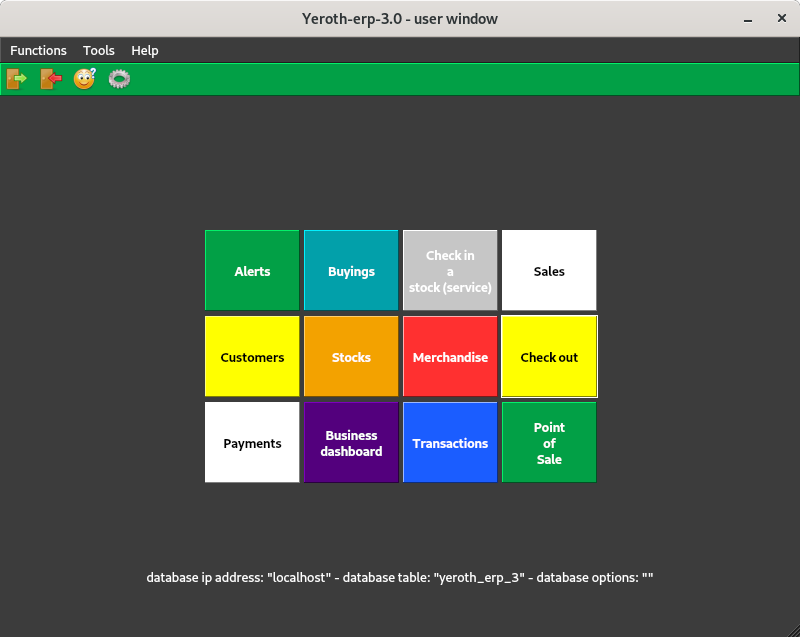
\includegraphics[scale=0.25]{images/yeroth-manager-window.png}
\caption*{Business manager's main window}

\vspace{3em}

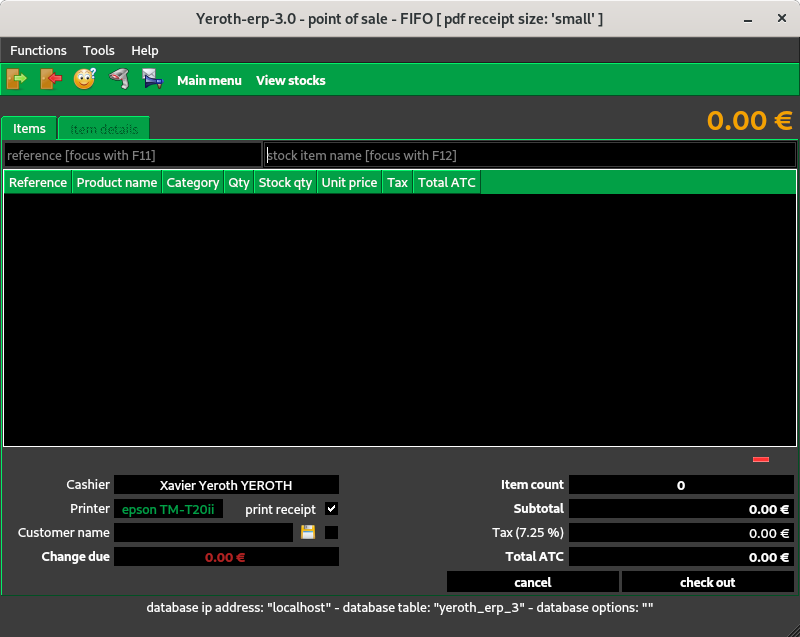
\includegraphics[scale=0.25]{images/yeroth-cashier-window.png}
\caption*{Cashier's main window}

\end{center}
}
\end{tabular}
\end{table}

\vspace{1.0em}

{\large \bf OPERATIONS}

\vspace{0.75em}

\begin{table}[!htbp]
\begin{tabular}{lll}

\begin{tcolorbox}[width=14.3em, boxrule=0.01em, colback=white]
\textbf{Point--of--Sale Hardware}
\vspace{-1em}
\hrule
\vspace{0.75em}
\begin{itemize}[]
	\item[\mycheckmark{yerothColorDarkgray}] Barcode scanner
	\item[\mycheckmark{yerothColorDarkgray}] Thermal printer, etc.\\
\end{itemize}
\begin{center}
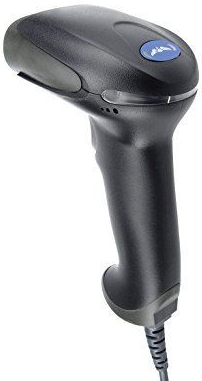
\includegraphics[scale=0.24]{images/xfox-fj-5-usb-plug-and-play-automatic-barcode-scanner.png}
\end{center}
\end{tcolorbox}

&

\begin{tcolorbox}[width=14.3em, boxrule=0.01em, colback=white]
\textbf{Database Management Systems}
\vspace{0.1em}
\hrule
\vspace{0.75em}
\begin{itemize}[]
	\item[\mycheckmark{yerothColorBlue}] \mysqlcolored\\
\end{itemize}
\begin{center}

\includegraphics[scale=0.14]{images/free-reuse-dbms-logo}
\end{center}
\end{tcolorbox}

&

\begin{tcolorbox}[width=14.3em, boxrule=0.01em, colback=white]
\textbf{Operating Systems}
\vspace{0.1em}
\hrule
\vspace{0.75em}
\begin{itemize}[]
	\item[\mycheckmark{yerothColorRed}] Debian--Linux\\	
\end{itemize}
\begin{center}

\includegraphics[scale=0.53]{images/free-reuse-stretch-logo}
\end{center}
\end{tcolorbox}

\end{tabular}
\end{table}
	
\end{document}

